% Options for packages loaded elsewhere
\PassOptionsToPackage{unicode}{hyperref}
\PassOptionsToPackage{hyphens}{url}
%
\documentclass[
]{book}
\usepackage{amsmath,amssymb}
\usepackage{lmodern}
\usepackage{iftex}
\ifPDFTeX
  \usepackage[T1]{fontenc}
  \usepackage[utf8]{inputenc}
  \usepackage{textcomp} % provide euro and other symbols
\else % if luatex or xetex
  \usepackage{unicode-math}
  \defaultfontfeatures{Scale=MatchLowercase}
  \defaultfontfeatures[\rmfamily]{Ligatures=TeX,Scale=1}
\fi
% Use upquote if available, for straight quotes in verbatim environments
\IfFileExists{upquote.sty}{\usepackage{upquote}}{}
\IfFileExists{microtype.sty}{% use microtype if available
  \usepackage[]{microtype}
  \UseMicrotypeSet[protrusion]{basicmath} % disable protrusion for tt fonts
}{}
\makeatletter
\@ifundefined{KOMAClassName}{% if non-KOMA class
  \IfFileExists{parskip.sty}{%
    \usepackage{parskip}
  }{% else
    \setlength{\parindent}{0pt}
    \setlength{\parskip}{6pt plus 2pt minus 1pt}}
}{% if KOMA class
  \KOMAoptions{parskip=half}}
\makeatother
\usepackage{xcolor}
\usepackage{longtable,booktabs,array}
\usepackage{calc} % for calculating minipage widths
% Correct order of tables after \paragraph or \subparagraph
\usepackage{etoolbox}
\makeatletter
\patchcmd\longtable{\par}{\if@noskipsec\mbox{}\fi\par}{}{}
\makeatother
% Allow footnotes in longtable head/foot
\IfFileExists{footnotehyper.sty}{\usepackage{footnotehyper}}{\usepackage{footnote}}
\makesavenoteenv{longtable}
\usepackage{graphicx}
\makeatletter
\def\maxwidth{\ifdim\Gin@nat@width>\linewidth\linewidth\else\Gin@nat@width\fi}
\def\maxheight{\ifdim\Gin@nat@height>\textheight\textheight\else\Gin@nat@height\fi}
\makeatother
% Scale images if necessary, so that they will not overflow the page
% margins by default, and it is still possible to overwrite the defaults
% using explicit options in \includegraphics[width, height, ...]{}
\setkeys{Gin}{width=\maxwidth,height=\maxheight,keepaspectratio}
% Set default figure placement to htbp
\makeatletter
\def\fps@figure{htbp}
\makeatother
\setlength{\emergencystretch}{3em} % prevent overfull lines
\providecommand{\tightlist}{%
  \setlength{\itemsep}{0pt}\setlength{\parskip}{0pt}}
\setcounter{secnumdepth}{5}
\usepackage{booktabs}
\ifLuaTeX
  \usepackage{selnolig}  % disable illegal ligatures
\fi
\usepackage[]{natbib}
\bibliographystyle{plainnat}
\IfFileExists{bookmark.sty}{\usepackage{bookmark}}{\usepackage{hyperref}}
\IfFileExists{xurl.sty}{\usepackage{xurl}}{} % add URL line breaks if available
\urlstyle{same} % disable monospaced font for URLs
\hypersetup{
  pdftitle={Pivot Tables in Excel},
  pdfauthor={Joe Hobart},
  hidelinks,
  pdfcreator={LaTeX via pandoc}}

\title{Pivot Tables in Excel}
\author{Joe Hobart}
\date{}

\begin{document}
\maketitle

{
\setcounter{tocdepth}{1}
\tableofcontents
}
\hypertarget{introduction}{%
\chapter{Introduction}\label{introduction}}

Pivot tables are a powerful tool for data analysis and visualization in various domains, ranging from business and finance to research and marketing. Here, we explore the intricacies of pivot tables, their functionality, and practical applications. We cover the basics of pivot tables including step-by-step instructions on creating and customizing them. We discuss advanced techniques for data manipulation and tips for optimizing their usage. By the end, our hope is that readers will have a solid understanding of pivot tables and be able to use them to derive meaningful insights from complex data.

\hypertarget{definition-and-purpose}{%
\section{Definition and Purpose}\label{definition-and-purpose}}

Pivot tables are a data summarization tool that allows users to extract meaningful insights from large datasets. They enable dynamic data analysis and manipulation, allowing users to reorganize and summarize data based on different criteria. Pivot tables provide a flexible and interactive way to explore data, identify patterns, and uncover trends that may not be immediately apparent.

\hypertarget{benefits-of-pivot-tables}{%
\section{Benefits of Pivot Tables}\label{benefits-of-pivot-tables}}

Pivot tables offer several advantages for data analysis:

\begin{itemize}
\tightlist
\item
  \textbf{Simplified Data Summarization:} Pivot tables provide a simplified way to summarize and aggregate large datasets into manageable and meaningful information.
\item
  \textbf{Dynamic Analysis:} Pivot tables allow users to change the layout and structure of the data on the fly, making it easy to explore different dimensions and perspectives.
\item
  \textbf{Interactive Exploration:} Pivot tables enable users to interactively drill down into the data, filter specific values, and perform ad-hoc analysis.
\item
  \textbf{Easy Customization:} Pivot tables offer various customization options, allowing users to tailor the analysis to their specific needs.
\item
  \textbf{Visual Representation:} Pivot tables can be visually enhanced with charts and graphs to facilitate data visualization and communication.
\end{itemize}

\hypertarget{pivot-table-components}{%
\section{Pivot Table Components}\label{pivot-table-components}}

The components of a pivot table are as follows:

\begin{itemize}
\tightlist
\item
  \textbf{Rows:} The row field(s) determine the arrangement of data in the rows of the pivot table. Each unique value in the row field(s) creates a separate row in the pivot table, and the data is organized accordingly.
\item
  \textbf{Columns:} The column field(s) determine the arrangement of data in the columns of the pivot table. Similar to the row field(s), each unique value in the column field(s) creates a separate column in the pivot table.
\item
  \textbf{Values:} The value field(s) contain the data that is summarized and displayed within the pivot table. These values are typically numeric or measurable data, such as sales figures, quantities, or percentages. The aggregation function applied to the value field(s) determines how the data is summarized (e.g., sum, average, count).
\item
  \textbf{Report Filters:} Report filters allow users to filter the data displayed in the pivot table based on specific criteria. By selecting or deselecting filter options, users can focus on specific subsets of data, making it easier to analyze and draw insights.
\end{itemize}

In summary, the row and column fields determine the structure of the pivot table, the value field(s) contain the data to be summarized, and the report filters allow for further data filtering and analysis. Together, these components provide a flexible and interactive way to explore and analyze complex datasets.

\hypertarget{getting-started-with-pivot-tables}{%
\chapter{Getting Started with Pivot Tables}\label{getting-started-with-pivot-tables}}

\hypertarget{data-requirements}{%
\section{Data Requirements}\label{data-requirements}}

Before creating a pivot table, it is crucial to ensure that your data meets certain requirements. These requirements include:

\begin{itemize}
\tightlist
\item
  \textbf{Data Format:} Data must be organized in a tabular format, with each column representing a specific variable and each row containing a unique record.
\item
  \textbf{Column Headers:} Ensure that your data have unique column headers. These headers will be used as field names in the pivot table.
\item
  \textbf{Consistent Data Types:} Each column has a consistent data types. For example, numeric columns should contain only numbers, date columns should contain only dates, and text columns should contain only text values. Inconsistent data types may lead to incorrect calculations or unexpected results in the pivot table.
\item
  \textbf{No Blank Cells:} Blank cells can disrupt the calculations performed by the pivot table and may result in inaccurate summaries. Therefore, blank cells need to be removed or imputed.
\end{itemize}

\hypertarget{preparing-the-data}{%
\section{Preparing the Data}\label{preparing-the-data}}

To ensure that your data is ready for pivot table analysis, consider the following preparation steps:

\begin{itemize}
\tightlist
\item
  \textbf{Data Cleaning:} Clean the data by removing any duplicates, correcting errors, and handling missing values. This process enhances the accuracy and reliability of the analysis performed by the pivot table.
\item
  \textbf{Data Consolidation:} If your data is scattered across multiple worksheets, consolidate it into a single location. This ensures that all relevant data is included in the analysis.
\item
  \textbf{Data Transformation:} Depending on your analysis objectives, you may need to transform your data before creating a pivot table. For example, you might want to convert text values to numerical values or split a single column into multiple columns.
\end{itemize}

\hypertarget{creating-a-pivot-table-in-excel}{%
\section{Creating a Pivot Table in Excel}\label{creating-a-pivot-table-in-excel}}

Excel provides a user-friendly interface for creating pivot tables. Follow these steps to create a pivot table:

Step 1: Select your Data Range: Highlight the range of cells that contain your data, including the column headers.

Step 2: Insert a Pivot Table: Navigate to the ``Insert'' tab in the Excel ribbon and click on the ``PivotTable'' button. This will open the ``Create PivotTable'' dialog box.

Step 3: Choose the Data Source: In the ``Create PivotTable'' dialog box, verify that the ``Select a table or range'' option is selected. Ensure that the correct data range is displayed in the ``Table/Range'' field. If your data range includes column headers, Excel will automatically detect them.

Step 4: Select the Pivot Table Destination: Choose where you want to place the pivot table. You can either select an existing worksheet or create a new worksheet. Once you've made your selection, click ``OK.''

Step 5: Design the Pivot Table: Excel will open a new worksheet or insert a pivot table within an existing worksheet. On the right side of the Excel window, you will see the ``PivotTable Fields'' pane. This pane displays a list of all the fields (columns) from your data range.

\hypertarget{a-pivot-table-example}{%
\section{A Pivot Table Example}\label{a-pivot-table-example}}

Download the file ``PivotTableData1'' from \href{https://github.com/JoeH123/Data}{here}. Do this by clicking on the file ``PivotTableData1.xlsx'', then click ``View raw'' to download the dataset.

This dataset gives enrollment statistics for various classes in Mathematics, Statistics and Data Science.

We will recreate the pivot table seen below.

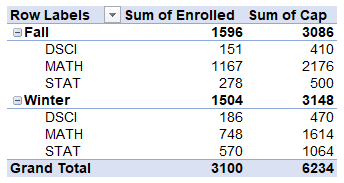
\includegraphics{PT1.png}

\begin{enumerate}
\def\labelenumi{\arabic{enumi}.}
\tightlist
\item
  Begin by highlighting the data.
\item
  Under ``Insert'', click ``Pivot Table''.
\item
  Verify the settings in the pivot table dialogue box are what you want. In this case, the defaults are fine. Click ``OK''.
\item
  Drag the ``Term'' field under ``Rows''.
\item
  Drag the ``Subj'' field under ``Rows''.
\item
  Drag the ``Enrolled'' field under ``Values''.
\item
  Drag the ``Cap'' field under ``Values''.
\end{enumerate}

Notice that the ``columns'' area automatically adds a ``sum Values'' field. So, in this case, we are adding up the enrollments and capacity from the classes in the various subject areas.

\hypertarget{pivot-table-layout-and-structure}{%
\section{Pivot Table Layout and Structure}\label{pivot-table-layout-and-structure}}

Once you have created a pivot table in Excel, it is important to understand its layout and structure. A pivot table consists of several key elements that allow you to organize, summarize, and analyze your data effectively.

\begin{enumerate}
\def\labelenumi{\arabic{enumi}.}
\item
  PivotTable Fields Pane:
  The PivotTable Fields pane is located on the right side of the Excel window when a pivot table is active. It displays a list of all the fields (columns) from your data range. The fields are categorized into four sections: Filters, Columns, Rows, and Values.

  \begin{itemize}
  \tightlist
  \item
    Filters: The fields placed in the Filters section allow you to filter the data displayed in the pivot table based on specific criteria. You can select or deselect values in the filter drop-down to focus on specific subsets of data.
  \item
    Columns: The fields placed in the Columns section determine the arrangement of data in the columns of the pivot table. Each unique value in the column field(s) creates a separate column in the pivot table.
  \item
    Rows: The fields placed in the Rows section determine the arrangement of data in the rows of the pivot table. Each unique value in the row field(s) creates a separate row in the pivot table.
  \item
    Values: The fields placed in the Values section contain the data that is summarized and displayed within the pivot table. These values are typically numeric or measurable data, such as sales figures, quantities, or percentages. You can apply various aggregation functions to the value field(s), such as sum, average, count, etc., to calculate summary statistics.
  \end{itemize}
\item
  PivotTable Field List:
  The PivotTable Field List is a floating window that appears when you click inside the pivot table. It provides a more detailed view of the fields and allows you to make changes to the pivot table structure. You can drag and drop fields between the Filters, Columns, Rows, and Values sections to modify the layout and analysis perspective of the pivot table.
\item
  PivotTable Tools:
  When you click inside the pivot table, a new tab called ``PivotTable Tools'' appears in the Excel ribbon. This tab contains two sub-tabs: Analyze and Design. These tabs provide additional options and functionalities to customize and enhance the pivot table.

  \begin{itemize}
  \tightlist
  \item
    Analyze Tab: The Analyze tab allows you to modify the pivot table layout, apply different calculations, sort and filter data, and format the pivot table. It provides tools for refreshing the data, changing the pivot table layout, adding calculated fields, and more.
  \item
    Design Tab: The Design tab offers various customization options to change the appearance and style of the pivot table. You can choose from different predefined pivot table styles, modify field settings, add subtotals and grand totals, and format the pivot table with different themes, colors, and fonts.
  \end{itemize}
\item
  Pivot Table Cells:
  The main body of the pivot table consists of cells that display the summarized data. Each cell represents the intersection of a row field and a column field. The values in these cells are calculated based on the aggregation function applied to the value field(s). You can also apply conditional formatting to highlight specific data patterns or set up data bars, color scales, or icon sets to visualize the data within the cells.
\item
  Drill-Down and Expand/Collapse:
  One of the powerful features of pivot tables is the ability to drill down into the data and expand or collapse the levels of detail. By double-clicking a cell in the pivot table, you can access the underlying data that makes up that specific value. Additionally, you can expand or collapse the row or column field headers to show or hide the detailed data for specific categories or groups.
\end{enumerate}

Understanding the layout and structure of a pivot table allows you to manipulate and analyze data efficiently. By utilizing the PivotTable Fields pane, PivotTable Field
List, PivotTable Tools, and various customization options, you can create dynamic and insightful pivot tables to derive meaningful insights from your data.

\hypertarget{another-example}{%
\section{Another Example}\label{another-example}}

Download the file ``PivotTableData1'' from \href{https://github.com/JoeH123/Data}{here}. Do this by clicking on the file ``PivotTableData1.xlsx'', then click ``View raw'' to download the dataset.

This dataset gives enrollment statistics for various classes in Mathematics, Statistics and Data Science.

We will recreate the pivot table seen below.

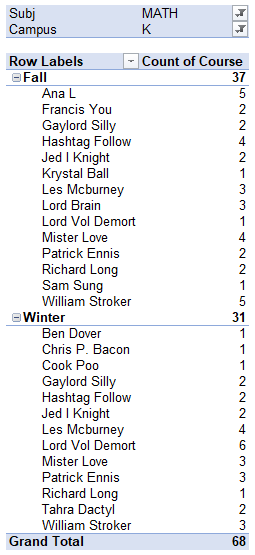
\includegraphics{PT2.png}

\begin{enumerate}
\def\labelenumi{\arabic{enumi}.}
\tightlist
\item
  Begin by highlighting the data.
\item
  Under ``Insert'', click ``Pivot Table''.
\item
  Verify the settings in the pivot table dialogue box are what you want. In this case, the defaults are fine. Click ``OK''.
\item
  Drag the ``Term'' field under ``Rows''.
\item
  Drag the ``Instructor'' field under ``Rows''.
\item
  Drag the ``Subj'' field under ``Filters''.
\item
  Drag the ``Campus'' field under ``Filters''.
\item
  Drag the ``Course'' field under ``Values''.
\end{enumerate}

Now, we have a count of how many courses each instructor teaches. In the pivot table, click on the ``Subj'' filter and select ``MATH''. Click on the ``Campus'' filter and select ``K''. This filters the list to instructors who teach classes in MATH at campus K.

\hypertarget{pivot-table-fields-and-values}{%
\chapter{Pivot Table Fields and Values}\label{pivot-table-fields-and-values}}

Pivot table fields and values are fundamental components that define the structure and analysis of pivot tables. In this section, we delve into the details of row fields, column fields, value fields, and report filters. We explore how each of these elements contributes to the organization, summarization, and manipulation of data within pivot tables. By understanding the capabilities and options available for pivot table fields and values, readers will gain a solid foundation to leverage the full potential of pivot tables in their data analysis endeavors.

\hypertarget{row-fields}{%
\section{Row Fields}\label{row-fields}}

\hypertarget{what-are-row-fields}{%
\subsection{What are Row Fields?}\label{what-are-row-fields}}

Row fields determine the arrangement of data in the rows of a pivot table. Each unique value in a row field creates a separate row in the pivot table, facilitating data grouping and segmentation. We explore the concept of row fields in detail, including how to add, remove, and rearrange them, as well as techniques for expanding and collapsing data at different levels of detail.

\hypertarget{adding-row-fields}{%
\subsection{Adding Row Fields}\label{adding-row-fields}}

To add a row field to a pivot table in Excel, you can simply drag and drop a column header from the PivotTable Field List into the ``Rows'' section of the PivotTable Fields pane. Alternatively, you can check the box next to the desired field name in the PivotTable Field List to include it as a row field.

\hypertarget{organizing-data-with-row-fields}{%
\subsection{Organizing Data with Row Fields}\label{organizing-data-with-row-fields}}

Row fields provide a way to organize and structure data in a pivot table. They allow you to group data by various categories or dimensions, providing a hierarchical structure for analysis. For example, in a sales dataset, you might have row fields such as ``Region,'' ``Product Category,'' and ``Sales Representative.'' This arrangement allows you to examine sales performance by region, product category, and individual sales representatives.

\hypertarget{expanding-and-collapsing-row-fields}{%
\subsection{Expanding and Collapsing Row Fields}\label{expanding-and-collapsing-row-fields}}

One of the key features of row fields is the ability to expand and collapse the levels of detail in a pivot table. By clicking the small plus or minus icons next to a row field, you can expand or collapse the data at different levels of detail. This functionality is useful when dealing with large datasets, as it allows you to focus on specific subsets of data or obtain a more comprehensive view of the information.

\hypertarget{sorting-and-filtering-row-fields}{%
\subsection{Sorting and Filtering Row Fields}\label{sorting-and-filtering-row-fields}}

Excel provides options to sort and filter data within row fields. By right-clicking on a row label or using the Sort and Filter options in the ribbon, you can rearrange the order of rows based on specific criteria or apply filters to display only relevant data. Sorting and filtering row fields help in identifying trends, outliers, or specific data subsets that require further analysis.

\hypertarget{customizing-row-field-settings}{%
\subsection{Customizing Row Field Settings}\label{customizing-row-field-settings}}

Excel offers various customization options for row fields in pivot tables. You can adjust the field settings to control how data is displayed within the rows. For instance, you can choose to show or hide subtotals, modify the number format, change the layout, and customize the appearance of the row labels. These settings allow you to present data in a format that best suits your analytical needs.

\hypertarget{summary-totals-in-row-fields}{%
\subsection{Summary Totals in Row Fields}\label{summary-totals-in-row-fields}}

Row fields provide an automatic summary of values within each row, based on the selected value fields. Excel offers various aggregation functions, such as sum, count, average, min, max, etc., that calculate the summary totals for the data. This feature allows you to quickly analyze and compare data across different row categories.

\hypertarget{nested-row-fields}{%
\subsection{Nested Row Fields}\label{nested-row-fields}}

In more complex datasets, you may need to create nested row fields, where one field is nested within another. This allows for a more detailed analysis and breakdown of data. For example, you can have a row field for ``Year'' and nest another row field for ``Quarter'' within it. This arrangement provides a hierarchical view of data, enabling you to explore trends and patterns at different levels of granularity.

\hypertarget{drill-down-analysis}{%
\subsection{Drill-Down Analysis}\label{drill-down-analysis}}

Row fields support drill-down analysis, allowing you to explore the underlying data within a specific row. By double-clicking on a row value, you can drill down into the data and view the individual records that contribute to that particular row. This feature is valuable when you want to investigate anomalies, identify contributing factors, or perform a more granular analysis of the data.

\hypertarget{example}{%
\subsection{Example}\label{example}}

Recreate the pivot table below.

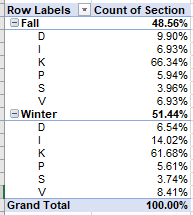
\includegraphics{PT4.png}

\hypertarget{column-fields}{%
\section{Column Fields}\label{column-fields}}

\hypertarget{what-are-column-fields}{%
\subsection{What are Column Fields?}\label{what-are-column-fields}}

Column fields determine the arrangement of data in the columns of a pivot table. Similar to row fields, each unique value in a column field creates a separate column in the pivot table, enabling data analysis from different perspectives. We discuss the usage of column fields, including techniques for adding, removing, and rearranging them to generate desired columnar representations of data.

\hypertarget{adding-column-fields}{%
\subsection{Adding Column Fields}\label{adding-column-fields}}

To add a column field to a pivot table, you can simply drag and drop a column header from the PivotTable Field List into the ``Columns'' section of the PivotTable Fields pane. Alternatively, you can check the box next to the desired field name in the PivotTable Field List to include it as a column field.

\hypertarget{analyzing-data-with-column-fields}{%
\subsection{Analyzing Data with Column Fields}\label{analyzing-data-with-column-fields}}

Column fields allow for a more in-depth analysis of data in pivot tables. By incorporating column fields, you can segment and compare data across different categories or dimensions. For instance, in a sales dataset, you might have column fields such as ``Product Category,'' ``Month,'' or ``Region.'' This arrangement facilitates the examination of sales performance by product category, month, or region, enabling you to identify patterns and trends.

\hypertarget{expanding-and-collapsing-column-fields}{%
\subsection{Expanding and Collapsing Column Fields}\label{expanding-and-collapsing-column-fields}}

Similar to row fields, column fields offer the flexibility to expand or collapse levels of detail within a pivot table. By clicking the plus or minus icons next to a column field, you can expand or collapse the data at different levels, adjusting the level of granularity in the analysis. This feature is particularly useful when dealing with large datasets or when you want to focus on specific subsets of data.

\hypertarget{sorting-and-filtering-column-fields}{%
\subsection{Sorting and Filtering Column Fields}\label{sorting-and-filtering-column-fields}}

Excel provides options to sort and filter data within column fields. By right-clicking on a column label or using the Sort and Filter options in the ribbon, you can rearrange the order of columns based on specific criteria or apply filters to display only relevant data. Sorting and filtering column fields enable you to examine data in a customized manner and highlight specific trends or outliers.

\hypertarget{customizing-column-field-settings}{%
\subsection{Customizing Column Field Settings}\label{customizing-column-field-settings}}

Excel offers various customization options for column fields in pivot tables. You can modify the field settings to control how data is displayed within the columns. For instance, you can choose to show or hide subtotals, adjust the number format, change the layout, and customize the appearance of the column labels. These settings allow you to present data in a format that best suits your analytical needs and enhances data visualization.

\hypertarget{grouping-data-with-column-fields}{%
\subsection{Grouping Data with Column Fields}\label{grouping-data-with-column-fields}}

Column fields can be utilized to group data into meaningful categories, simplifying the analysis and presentation of complex datasets. Excel provides the option to group dates, numbers, or text values within column fields. For example, you can group sales data by quarters or group product prices into price ranges. Grouping data enhances the clarity and organization of the pivot table, enabling easier interpretation and comparison of data.

\hypertarget{calculations-within-column-fields}{%
\subsection{Calculations within Column Fields}\label{calculations-within-column-fields}}

Excel pivot tables offer the ability to perform calculations within column fields. You can add calculated fields that derive new values based on existing data. This feature allows you to apply mathematical operations, perform comparisons, or create custom calculations to obtain additional insights. Calculated fields within column fields provide a flexible way to incorporate calculated data elements in your analysis.

\hypertarget{advanced-column-field-techniques}{%
\subsection{Advanced Column Field Techniques}\label{advanced-column-field-techniques}}

Excel provides advanced techniques for column fields, including the use of slicers and timelines. Slicers enable interactive filtering by providing visual buttons that represent different values within a column field. Timelines, specifically useful for date-based data, provide an intuitive interface for filtering and analyzing time-based data in columns. These features enhance the interactivity and flexibility of column fields, making data exploration and analysis more dynamic.

\hypertarget{example-1}{%
\subsection{Example}\label{example-1}}

Recreate the pivot table below.

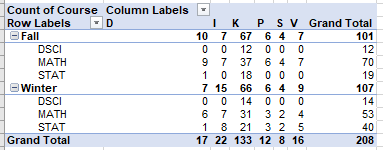
\includegraphics{PT5.png}

\hypertarget{value-fields}{%
\section{Value Fields}\label{value-fields}}

\hypertarget{understanding-value-fields}{%
\subsection{Understanding Value Fields}\label{understanding-value-fields}}

Value fields in Excel pivot tables contain the data that is summarized and displayed within the pivot table. These fields typically consist of numeric or measurable data, such as sales figures, quantities, or percentages. Value fields serve as the foundation for calculations and aggregations, providing a comprehensive overview of the data.

\hypertarget{adding-value-fields}{%
\subsection{Adding Value Fields}\label{adding-value-fields}}

To add a value field to a pivot table, you can drag and drop a column header from the PivotTable Field List into the ``Values'' section of the PivotTable Fields pane. Alternatively, you can check the box next to the desired field name in the PivotTable Field List to include it as a value field.

\hypertarget{aggregating-data-with-value-fields}{%
\subsection{Aggregating Data with Value Fields}\label{aggregating-data-with-value-fields}}

Value fields allow for the aggregation and summarization of data within pivot tables. Excel provides various aggregation functions, including sum, count, average, min, max, and more. These functions calculate the summary values based on the data in the value field. For example, you can sum the sales figures, count the number of transactions, or calculate the average price.

\hypertarget{customizing-value-field-settings}{%
\subsection{Customizing Value Field Settings}\label{customizing-value-field-settings}}

Excel offers customization options for value fields, allowing you to control how the data is summarized and displayed in the pivot table. You can adjust settings such as number format, decimal places, and display options for subtotals and grand totals. These settings enable you to present the data in a format that best suits your analysis and reporting requirements.

\hypertarget{value-field-summarization}{%
\subsection{Value Field Summarization}\label{value-field-summarization}}

Excel provides flexibility in summarizing value fields within pivot tables. You can choose to display the summarization as sums, averages, counts, percentages, or other applicable calculations. Depending on the nature of your data and analysis objectives, you can select the appropriate summarization function to obtain the desired insights.

\hypertarget{multiple-value-fields}{%
\subsection{Multiple Value Fields}\label{multiple-value-fields}}

Pivot tables allow you to include multiple value fields, enabling you to analyze and compare multiple aspects of the data simultaneously. For instance, you can include sales figures and profit margins as separate value fields to gain a comprehensive understanding of the financial performance. The ability to incorporate multiple value fields enhances the depth and breadth of analysis within pivot tables.

\hypertarget{calculated-fields-with-value-fields}{%
\subsection{Calculated Fields with Value Fields}\label{calculated-fields-with-value-fields}}

Excel pivot tables offer the option to create calculated fields based on the existing value fields. Calculated fields allow you to perform additional calculations and derive new insights from the data. You can create formulas using operators, functions, and references to other value fields within the pivot table. Calculated fields provide a flexible way to incorporate custom calculations and perform complex analysis.

\hypertarget{formatting-and-conditional-formatting}{%
\subsection{Formatting and Conditional Formatting}\label{formatting-and-conditional-formatting}}

Excel provides formatting options to enhance the visual presentation of value fields within pivot tables. You can apply number formatting, such as currency, percentage, or scientific notation, to improve readability. Additionally, conditional formatting allows you to highlight specific data patterns, trends, or outliers based on predefined rules or custom conditions. These formatting options aid in data visualization and emphasize key insights.

\hypertarget{filtering-and-sorting-value-fields}{%
\subsection{Filtering and Sorting Value Fields}\label{filtering-and-sorting-value-fields}}

Value fields can be filtered and sorted within pivot tables to focus on specific subsets of data or identify trends. Excel provides filtering options that allow you to display or hide specific values, apply top/bottom filters, or use custom filters to select data based on specific criteria. Sorting value fields in ascending or descending order helps identify the highest or lowest values, enabling you to analyze the data more effectively.

\hypertarget{drill-down-analysis-with-value-fields}{%
\subsection{Drill-Down Analysis with Value Fields}\label{drill-down-analysis-with-value-fields}}

Value fields support drill-down analysis within pivot tables. By double-clicking on a value in the pivot table, you can access the underlying data that contributes to that value. This feature is useful when you want to investigate the details of specific aggregated values, such as exploring the individual transactions that make up a total sales figure. Drill-down analysis allows for a more granular examination of the data and facilitates data exploration.

\hypertarget{example-2}{%
\subsection{Example}\label{example-2}}

Recreate the pivot table below.

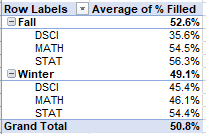
\includegraphics{PT6.png}

\hypertarget{report-filters}{%
\section{Report Filters}\label{report-filters}}

Report filters provide a means to filter the data displayed in a pivot table based on specific criteria. By applying report filters, users can focus on subsets of data that are relevant to their analysis, enabling more targeted and specific insights. We discuss the concept of report filters, including how to add, remove, and customize them, as well as techniques for applying multiple filters and utilizing advanced filtering options.

\hypertarget{adding-report-filters}{%
\subsection{Adding Report Filters}\label{adding-report-filters}}

To add a report filter to a pivot table, you can drag and drop a column header from the PivotTable Field List into the ``Report Filters'' section of the PivotTable Fields pane. Alternatively, you can check the box next to the desired field name in the PivotTable Field List to include it as a report filter.

\hypertarget{applying-report-filters}{%
\subsection{Applying Report Filters}\label{applying-report-filters}}

Once a report filter is added to a pivot table, you can use it to filter the data displayed in the pivot table. Excel provides various options for applying report filters. You can select or deselect specific values in the filter drop-down menu to include or exclude them from the analysis. Additionally, you can apply multiple report filters to further refine the data.

\hypertarget{filtering-numeric-and-date-fields}{%
\subsection{Filtering Numeric and Date Fields}\label{filtering-numeric-and-date-fields}}

Report filters offer specialized filtering options for numeric and date fields. For numeric fields, Excel provides filtering options such as equal to, not equal to, greater than, less than, and between. This allows you to narrow down the data based on specific numeric criteria. Similarly, for date fields, you can apply filters based on a specific date, date range, or other conditions.

\hypertarget{customizing-report-filter-settings}{%
\subsection{Customizing Report Filter Settings}\label{customizing-report-filter-settings}}

Excel offers customization options for report filters to enhance their functionality and appearance. You can modify the filter settings to control how the data is displayed and filtered. For example, you can show or hide items with no data, display items in alphabetical or custom order, or sort items based on specific criteria. These settings enable you to customize the report filter behavior according to your analysis requirements.

\hypertarget{slicers-for-enhanced-filtering}{%
\subsection{Slicers for Enhanced Filtering}\label{slicers-for-enhanced-filtering}}

Slicers are an alternative way to apply report filters in pivot tables. They provide a visual and user-friendly interface for filtering data. Slicers are interactive buttons or menus that represent different values within a report filter. By selecting or deselecting slicer buttons, you can dynamically filter the data displayed in the pivot table. Slicers enhance the visual experience and make filtering more intuitive.

\hypertarget{using-timelines-for-date-filtering}{%
\subsection{Using Timelines for Date Filtering}\label{using-timelines-for-date-filtering}}

Timelines are a specialized type of slicer designed specifically for date fields. They provide an intuitive and interactive way to filter and analyze time-based data within a pivot table. Timelines enable you to easily select specific time periods, such as months, quarters, or years, and visualize the filtered data. Timelines enhance the analysis of time series data and make it easier to identify trends and patterns.

\hypertarget{grouping-and-hierarchical-filtering}{%
\subsection{Grouping and Hierarchical Filtering}\label{grouping-and-hierarchical-filtering}}

Excel pivot tables allow you to group and hierarchically filter data based on report filters. You can group data within report filters to create logical categories or groupings. For example, you can group products by categories or group regions by territories. This grouping functionality enables a more organized and structured analysis, particularly for large datasets with numerous values.

\hypertarget{dynamic-filtering-and-interactive-analysis}{%
\subsection{Dynamic Filtering and Interactive Analysis}\label{dynamic-filtering-and-interactive-analysis}}

Report filters provide dynamic filtering capabilities within pivot tables. You can modify report filter selections on the fly to instantly update the data displayed in the pivot table. This interactivity allows for real-time exploration and analysis of the data. By adjusting the report filter criteria, you can dynamically observe the impact on the summarized data, enabling quick and interactive data analysis.

\hypertarget{filtering-best-practices}{%
\subsection{Filtering Best Practices}\label{filtering-best-practices}}

To maximize the effectiveness of report filters, it is important to follow best practices. These include keeping your data updated, refreshing pivot tables when necessary, using clear and descriptive field names, and utilizing efficient filtering techniques to focus on relevant data subsets. By adhering to these practices, you can ensure accurate and meaningful analysis using report filters.

\hypertarget{example-3}{%
\subsection{Example}\label{example-3}}

Recreate the pivot table below.

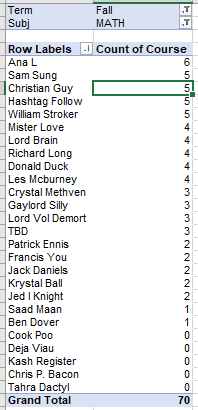
\includegraphics{PT3.png}

\hypertarget{customizing-pivot-tables}{%
\chapter{Customizing Pivot Tables}\label{customizing-pivot-tables}}

Pivot tables are powerful tools for data analysis and visualization in Excel. They provide a dynamic and flexible way to summarize and explore large datasets. However, to truly harness the potential of pivot tables, it is essential to understand how to customize them. This section will guide you through the process of customizing pivot tables, covering various aspects such as changing field settings, grouping data, sorting and filtering, and formatting pivot tables. By mastering these customization techniques, you can tailor pivot tables to meet your specific analysis and presentation needs.

\hypertarget{changing-field-settings}{%
\section{Changing Field Settings}\label{changing-field-settings}}

Changing field settings allows you to control how the data is summarized and displayed within the pivot table. Excel offers various options to modify field settings for row fields, column fields, and value fields.

\hypertarget{accessing-field-settings}{%
\subsection{Accessing Field Settings}\label{accessing-field-settings}}

To change field settings in a pivot table, you need to access the PivotTable Field List. This can be done by clicking anywhere inside the pivot table, which activates the PivotTable Tools in the Excel ribbon. From the Analyze or Options tab, click on the ``Field List'' button to display the PivotTable Field List pane. The field list contains all the available fields from your data source that can be added to the pivot table.

\hypertarget{modifying-value-field-settings}{%
\subsection{Modifying Value Field Settings}\label{modifying-value-field-settings}}

Value fields in a pivot table contain the data that is summarized and displayed within the table. Excel provides several options to modify the settings of value fields:

\begin{itemize}
\item
  Summarization Function: By default, Excel applies the ``Sum'' function to numeric value fields. However, you can change the summarization function to suit your analysis needs. Right-click on a value field in the pivot table, select ``Value Field Settings,'' and choose a different function such as count, average, minimum, maximum, or a custom calculation.
\item
  Number Format: You can also modify the number format of the values displayed in the pivot table. Right-click on a value field, select ``Value Field Settings,'' and click on the ``Number Format'' button. From here, you can choose the desired format, such as currency, percentage, scientific notation, or custom formats.
\item
  Custom Calculations: In addition to the built-in summarization functions, Excel allows you to create custom calculations based on the existing value fields. This can be done by adding a calculated field to the pivot table. From the PivotTable Field List, click on the ``Fields, Items \& Sets'' button and select ``Calculated Field.'' Here, you can define a formula using operators, functions, and references to other value fields.Here are some key customization options:
\item
  Subtotals and Grand Totals: Excel allows you to control the display of subtotals and grand totals. You can choose to show or hide subtotals at different levels and include or exclude grand totals in the pivot table.
\end{itemize}

\hypertarget{field-settings-best-practices}{%
\subsection{Field Settings Best Practices}\label{field-settings-best-practices}}

To make the most of field settings in a pivot table, consider the following best practices:

\begin{itemize}
\item
  Understand Your Analysis Needs: Before modifying field settings, have a clear understanding of the analysis objectives and the insights you want to derive from the data. This will help you make informed decisions about the summarization functions, number formats, and custom calculations.
\item
  Test and Iterate: It is often beneficial to experiment with different field settings to find the most suitable configuration for your analysis. Don't hesitate to try different summarization functions, grouping options, or formatting styles until you achieve the desired results.
\item
  Document and Share: Once you have customized the field settings in a pivot table, consider documenting the changes or saving them as a template for future use. This will allow you to replicate the analysis or share it with others while maintaining consistency.
\end{itemize}

\hypertarget{grouping-data}{%
\section{Grouping Data}\label{grouping-data}}

Grouping data within pivot tables provides a way to organize and categorize information. Excel offers grouping options for both row fields and column fields. Here are the main grouping techniques:

\begin{itemize}
\item
  Date and Time Grouping: You can group date and time fields into predefined intervals such as days, months, quarters, or years. This simplifies the analysis of time-series data and enables you to identify patterns and trends more easily.
\item
  Numeric Grouping: For numeric fields, you can create custom groups or intervals to group values based on specific criteria. This allows for a more structured analysis, particularly when dealing with continuous data.
\item
  Hierarchical Grouping: Excel allows you to create hierarchical groups by nesting one field within another. For example, you can group products by category and then by subcategory. This hierarchical grouping provides a more detailed and organized view of the data.
\end{itemize}

\hypertarget{understanding-grouping-data-in-a-pivot-table}{%
\subsection{Understanding Grouping Data in a Pivot Table}\label{understanding-grouping-data-in-a-pivot-table}}

Grouping data in a pivot table involves combining individual values into categories or hierarchies based on specific criteria. It allows you to organize and present data in a more meaningful and structured manner. Grouping can be applied to both row fields and column fields, enabling you to create a hierarchical view of the data.

\hypertarget{grouping-date-and-time-data}{%
\subsection{Grouping Date and Time Data}\label{grouping-date-and-time-data}}

One common scenario for grouping data in a pivot table is working with date and time fields. Excel provides various grouping options for date and time data, including:

\begin{itemize}
\item
  Grouping by Days, Months, Quarters, or Years: You can group date fields into meaningful intervals such as days, months, quarters, or years. This allows for a higher-level analysis of trends and patterns over time.
\item
  Custom Date Grouping: Excel also allows you to define custom groupings for date fields. For example, you can group dates by specific periods, like fiscal weeks or marketing campaign durations. This level of customization provides more flexibility in analyzing data based on specific business needs.
\item
  Grouping Time Data: Similar to date grouping, you can group time fields into intervals such as hours, minutes, or seconds. This is useful when working with datasets that require more granular analysis based on time intervals.
\end{itemize}

\hypertarget{grouping-numeric-data}{%
\subsection{Grouping Numeric Data}\label{grouping-numeric-data}}

Grouping numeric data in a pivot table provides a way to create intervals or categories based on specific criteria. Some use cases for grouping numeric data include:

\begin{itemize}
\item
  Creating Age Ranges: When working with age data, you can group the values into ranges (e.g., 0-10, 11-20, etc.) to gain a better understanding of age distribution within the dataset.
\item
  Categorizing Numeric Values: Grouping numeric values allows you to create categories that make analysis easier. For instance, you can group sales figures into ranges to analyze sales performance based on different revenue segments.
\item
  Custom Numeric Grouping: Excel provides the flexibility to define custom numeric groupings based on specific requirements. This allows you to tailor the groupings to match your analysis needs and create more meaningful insights.
\end{itemize}

\hypertarget{grouping-text-data}{%
\subsection{Grouping Text Data}\label{grouping-text-data}}

Grouping text data in a pivot table is useful for categorizing or organizing information based on specific text values. Some scenarios where grouping text data is beneficial include:

\begin{itemize}
\item
  Categorizing Product Names: Grouping product names into specific categories helps in analyzing sales performance by product category. This grouping can be done based on common attributes or predefined categories.
\item
  Organizing Geographic Data: If your dataset includes geographic information, you can group locations by regions, countries, or other geographical divisions. This provides a higher-level overview of the data and simplifies analysis by geographic regions.
\item
  Grouping Other Textual Attributes: Grouping text data allows you to create logical categories for other attributes such as departments, customer segments, or job roles. This provides a more structured view of the data and helps in analyzing specific subsets of information.
\end{itemize}

\hypertarget{creating-hierarchies}{%
\subsection{Creating Hierarchies}\label{creating-hierarchies}}

Grouping data in a pivot table also allows you to create hierarchies, enabling a more detailed analysis. Hierarchies provide a structured and nested view of the data, allowing you to drill down into different levels of granularity. Some common hierarchies include:

\begin{itemize}
\item
  Date and Time Hierarchies: You can create date hierarchies by grouping fields at different levels, such as year, quarter, month, and day. This allows you to analyze data at various levels of time granularity.
\item
  Product Hierarchies: In sales or inventory datasets, you can create product hierarchies by grouping fields such as category, subcategory, and product name. This enables you to analyze sales performance at different levels of product categorization.
\item
  Geographic Hierarchies: Hierarchies can be created for geographic data by grouping fields such as region, country, and city. This allows you to drill down into specific geographic areas and analyze data accordingly.
\end{itemize}

\hypertarget{applying-multiple-groupings}{%
\subsection{Applying Multiple Groupings}\label{applying-multiple-groupings}}

Excel pivot tables allow you to apply multiple groupings simultaneously, providing a more comprehensive analysis. You can group data by multiple fields within the same row or column area. This allows for a multidimensional view of the data, enabling you to analyze different combinations of categories and hierarchies.

\hypertarget{dynamic-grouping}{%
\subsection{Dynamic Grouping}\label{dynamic-grouping}}

Dynamic grouping in a pivot table allows you to change the grouping options and update the pivot table dynamically. This is particularly useful when working with large datasets that require frequent adjustments to the grouping structure. With dynamic grouping, you can explore different perspectives of the data without recreating the entire pivot table.

\hypertarget{benefits-of-grouping-data-in-a-pivot-table}{%
\subsection{Benefits of Grouping Data in a Pivot Table}\label{benefits-of-grouping-data-in-a-pivot-table}}

Grouping data in a pivot table offers several benefits for data analysis:

\begin{itemize}
\item
  Enhanced Data Organization: Grouping data provides a logical and organized structure that improves the visual representation of the data. This allows for better understanding and interpretation of the information.
\item
  Simplified Analysis: Grouping allows you to condense large amounts of data into meaningful categories or hierarchies. This simplifies the analysis process and helps in identifying patterns, trends, and outliers more efficiently.
\item
  Improved Data Exploration: Grouping provides the flexibility to drill down into specific subsets of data within the pivot table. This enables a more granular analysis and the ability to explore the data from different angles.
\item
  Streamlined Reporting: Grouping data in a pivot table allows you to create concise and informative reports. By presenting data in a structured and categorized format, you can communicate insights effectively and support data-driven decision-making.
\end{itemize}

\hypertarget{sorting-and-filtering}{%
\section{Sorting and Filtering}\label{sorting-and-filtering}}

Sorting and filtering options in pivot tables allow you to organize and manipulate the data to focus on specific subsets. Here's how you can sort and filter pivot tables:

\hypertarget{sorting-data-in-a-pivot-table}{%
\subsection{Sorting Data in a Pivot Table}\label{sorting-data-in-a-pivot-table}}

Sorting data in a pivot table allows you to arrange information in a particular order based on selected criteria. Excel provides several sorting options for both row fields and column fields:

\begin{itemize}
\item
  Ascending and Descending Order: You can sort data in ascending (A to Z) or descending (Z to A) order. This is particularly useful when you want to identify the highest or lowest values within a field.
\item
  Value Sorting: Excel allows you to sort data based on the values within a field. You can sort by sum, average, count, minimum, maximum, or other applicable calculations. This sorting option helps in analyzing data based on specific aggregated values.
\item
  Manual Sorting: Manual sorting enables you to arrange data in a custom order. By clicking and dragging field items within the pivot table, you can rearrange them to meet your analysis requirements.
\end{itemize}

\hypertarget{filtering-data-in-a-pivot-table}{%
\subsection{Filtering Data in a Pivot Table}\label{filtering-data-in-a-pivot-table}}

Filtering data in a pivot table allows you to focus on specific subsets of information, enabling a more targeted analysis. Excel offers several filtering options for row fields, column fields, value fields, and report filters:

\begin{itemize}
\item
  Label Filters: Label filters allow you to filter data based on the values of a specific field. You can include or exclude specific values, filter by specific text, or apply conditions such as ``begins with,'' ``ends with,'' or ``contains.''
\item
  Value Filters: Value filters enable you to filter data based on specific criteria or conditions. You can filter data that meets certain numerical conditions, such as greater than, less than, between, or equal to a particular value.
\item
  Top/Bottom Filters: Top/bottom filters allow you to focus on a specified number or percentage of top or bottom values within a field. This is useful when you want to analyze the highest or lowest values within a dataset.
\item
  Multiple Filters: Excel pivot tables allow you to apply multiple filters simultaneously. By combining different filters using AND or OR operators, you can create complex filter criteria to refine your analysis.
\end{itemize}

\hypertarget{custom-filters-in-a-pivot-table}{%
\section{Custom Filters in a Pivot Table}\label{custom-filters-in-a-pivot-table}}

In addition to the standard filtering options, Excel provides custom filtering capabilities within a pivot table. Custom filters allow you to define specific filtering conditions based on your analysis requirements:

\begin{itemize}
\item
  Custom Text Filters: Custom text filters enable you to create custom filtering conditions using text criteria. This allows for more advanced text-based filtering, such as filtering data that contains specific words or phrases.
\item
  Custom Date Filters: Custom date filters allow you to define custom filtering conditions for date and time fields. You can filter data based on specific date ranges, periods, or relative dates.
\item
  Custom Number Filters: Custom number filters provide the flexibility to create custom filtering conditions based on numerical criteria. You can filter data based on specific ranges, greater than or less than values, or advanced calculations.
\end{itemize}

\hypertarget{sorting-and-filtering-best-practices}{%
\subsection{Sorting and Filtering Best Practices}\label{sorting-and-filtering-best-practices}}

To make the most of sorting and filtering in a pivot table, consider the following best practices:

\begin{itemize}
\item
  Understand Your Analysis Objectives: Before sorting and filtering data, have a clear understanding of your analysis objectives. Determine the specific insights you want to derive from the data, and identify the relevant sorting and filtering criteria.
\item
  Refresh and Update Data: It is essential to refresh and update the pivot table data regularly, especially when working with dynamic datasets. This ensures that the sorting and filtering reflect the latest information.
\item
  Utilize Multiple Sorting and Filtering Criteria: Instead of relying on a single sorting or filtering criterion, consider using multiple criteria to gain deeper insights. Combining different criteria allows you to focus on specific subsets of data and explore various aspects of your information.
\item
  Document Your Sorting and Filtering Choices: It is helpful to document the sorting and filtering choices you make in your pivot table. This allows you to replicate your analysis, track your decision-making process, and share your findings with others.
\end{itemize}

\hypertarget{sorting-and-filtering-report-filters}{%
\subsection{Sorting and Filtering Report Filters}\label{sorting-and-filtering-report-filters}}

Report filters are another powerful feature in pivot tables that allow you to filter data across the entire table. Sorting and filtering options for report filters work similarly to row and column fields, enabling you to narrow down the data displayed in the pivot table based on specific criteria.

\begin{itemize}
\item
  Sorting Report Filters: You can sort report filters alphabetically or numerically to arrange the filter values in a desired order. This makes it easier to locate specific values and navigate through the filter options.
\item
  Filtering Report Filters: Filtering report filters allows you to include or exclude specific values or apply custom filtering conditions. This helps in focusing the analysis on subsets of data that are relevant to your analysis objectives.
\end{itemize}

\hypertarget{clearing-sorting-and-filtering}{%
\subsection{Clearing Sorting and Filtering}\label{clearing-sorting-and-filtering}}

Excel provides options to clear sorting and filtering in a pivot table when you want to revert to the original state:

\begin{itemize}
\item
  Clear Sorting: To remove sorting from a field in a pivot table, you can click on the sort icon next to the field and select ``Clear Sort.''
\item
  Clear Filtering: To remove filtering from a field in a pivot table, you can click on the filter icon next to the field and select ``Clear Filter.''
\end{itemize}

\hypertarget{formatting-pivot-tables}{%
\subsection{Formatting Pivot Tables}\label{formatting-pivot-tables}}

Formatting is a crucial aspect of pivot table customization as it helps improve the visual appeal, readability, and overall presentation of the data. With Excel's extensive formatting options, you can enhance the appearance of your pivot tables and highlight key insights. In this section, we will explore the importance of formatting in a pivot table, discuss various formatting techniques, and provide practical tips for effective formatting.

\hypertarget{applying-pivot-table-styles}{%
\subsection{Applying Pivot Table Styles}\label{applying-pivot-table-styles}}

Pivot table styles are predefined formatting sets in Excel that provide a consistent and visually appealing look to the pivot table. Excel offers a variety of built-in styles that you can apply with a single click. Here are some key aspects of applying pivot table styles:

\begin{itemize}
\item
  Selecting a Style: To apply a pivot table style, select any cell within the pivot table, navigate to the PivotTable Tools Design tab in the Excel ribbon, and choose a style from the available options. Excel provides various styles with different color schemes, font styles, and border designs.
\item
  Modifying Style Elements: Pivot table styles are highly customizable. You can modify individual elements of a style, such as fonts, colors, shading, and borders. This allows you to tailor the style to match your specific preferences or branding requirements.
\item
  Creating Custom Styles: Excel also allows you to create custom pivot table styles by modifying existing styles or creating new ones from scratch. This feature provides flexibility in designing unique styles that suit your specific needs.
\end{itemize}

\hypertarget{cell-formatting-in-a-pivot-table}{%
\subsection{Cell Formatting in a Pivot Table}\label{cell-formatting-in-a-pivot-table}}

Cell formatting enables you to modify the appearance of individual cells within a pivot table. This helps in highlighting specific values, emphasizing key insights, or improving data readability. Here are some common cell formatting options:

\begin{itemize}
\item
  Font Formatting: Excel provides various font formatting options, including font type, size, color, and style (bold, italic, underline). You can modify the font formatting for specific cells or ranges within the pivot table to draw attention to important information.
\item
  Alignment and Indentation: Excel allows you to adjust the alignment and indentation of text within cells. You can align text to the left, center, or right of a cell and apply indentation for a more organized and structured presentation of data.
\item
  Number Formatting: Number formatting helps in displaying numeric values in a desired format, such as currency, percentage, decimal places, or scientific notation. By applying number formatting, you can improve the readability and interpretation of numeric data within the pivot table.
\item
  Conditional Formatting: Conditional formatting allows you to apply formatting rules based on specific conditions or criteria. This helps in visually highlighting patterns, trends, or outliers in the data. You can define custom rules or choose from a variety of predefined formatting options like color scales, data bars, icon sets, and more.
\end{itemize}

\hypertarget{charting-from-a-pivot-table}{%
\subsection{Charting from a Pivot Table}\label{charting-from-a-pivot-table}}

Charting is a powerful visualization tool that enables you to present data in a graphical format. Excel allows you to create various types of charts directly from a pivot table. Here's how you can chart from a pivot table:

\begin{itemize}
\item
  Selecting Data: Click on any cell within the pivot table, navigate to the PivotTable Tools Analyze or Options tab, and click on the ``PivotChart'' button. Excel will automatically select the pivot table data for chart creation.
\item
  Choosing a Chart Type: Excel offers a wide range of chart types, including column charts, bar charts, line charts, pie charts, and more. Select the chart type that best represents your data and analysis requirements.
\item
  Modifying Chart Elements: Once the chart is created, you can customize various chart elements such as titles, legends, axes, gridlines, data labels, and colors. Excel provides a set of formatting options that allow you to fine-tune the appearance of the chart to match your preferences.
\item
  Interacting with the Chart: Pivot charts are dynamic and interactive. You can drill down into the underlying data by clicking on chart elements, change chart views, and filter the data directly from the chart. This provides a more engaging and exploratory experience while analyzing the data.
\end{itemize}

\hypertarget{formatting-row-and-column-headers}{%
\subsection{Formatting Row and Column Headers}\label{formatting-row-and-column-headers}}

Row and column headers in a pivot table provide important contextual information about the data. Formatting these headers enhances the visual clarity and organization of the pivot table. Here are some formatting options for row and column headers:

\begin{itemize}
\item
  Font and Font Formatting: You can modify the font type, size, color, and style (bold, italic, underline) of the row and column headers. This allows you to emphasize the headers and improve their readability within the pivot table.
\item
  Background Color: Excel enables you to apply background colors or shading to the row and column headers. This helps in visually differentiating the headers from the data cells and improves the overall appearance of the pivot table.
\item
  Borders and Gridlines: Applying borders and gridlines to the row and column headers adds structure and delineation to the pivot table. Excel provides various border styles and thickness options that allow you to customize the appearance of the headers.
\end{itemize}

\hypertarget{example-4}{%
\subsection{Example}\label{example-4}}

Recreate the pivot tables below.

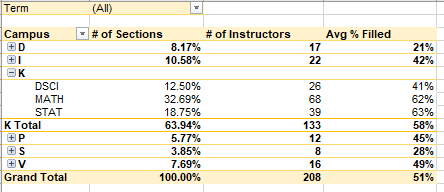
\includegraphics{PT7.png}

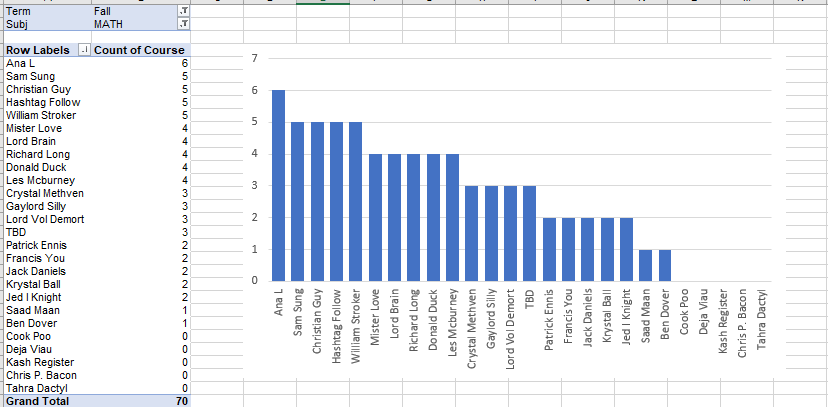
\includegraphics{PT8.png}

\hypertarget{aggregating-data-with-pivot-tables}{%
\chapter{Aggregating Data with Pivot Tables}\label{aggregating-data-with-pivot-tables}}

This chapter will delve into the various methods of aggregating data with pivot tables, covering key techniques such as summarizing data, counting and averaging data, calculating percentages and proportions, and working with dates and times. By understanding these aggregation methods, you will be able to derive valuable information from your data and make informed decisions.

\hypertarget{summarizing-data}{%
\section{Summarizing Data}\label{summarizing-data}}

Summarizing data is a fundamental function of pivot tables. It involves grouping and condensing data to provide an overview or total values for a specific category. Here are some key techniques for summarizing data:

\begin{itemize}
\item
  Summarization Functions: Pivot tables offer a variety of built-in summarization functions, such as sum, average, count, minimum, and maximum. These functions aggregate the data within a specific category or field. For example, if you have a sales dataset, you can use the sum function to calculate the total sales for each product or region.
\item
  Value Field Settings: Excel allows you to customize the summarization function for each value field in a pivot table. By right-clicking on a value field, selecting ``Value Field Settings,'' and choosing a different function, you can tailor the summarization method to meet your specific analysis needs.
\item
  Custom Calculations: If the built-in summarization functions do not fulfill your requirements, Excel provides the option to create custom calculations using calculated fields. This allows you to perform more complex calculations, derive new insights, or combine multiple value fields into a single aggregated value.
\end{itemize}

\hypertarget{counting-and-averaging-data}{%
\section{Counting and Averaging Data}\label{counting-and-averaging-data}}

Counting and averaging data are common operations when analyzing datasets. Pivot tables offer straightforward methods to count and average data based on specific criteria. Here's how you can use pivot tables to count and average data:

\begin{itemize}
\item
  Counting Data: To count the occurrences of data within a pivot table, add the desired field to the value area and change the summarization function to ``count.'' This will display the number of occurrences or records for each category or field. For instance, you can count the number of sales transactions for each product or the number of employees in each department.
\item
  Averaging Data: Pivot tables make it easy to calculate the average value of a dataset. By adding a field to the value area and changing the summarization function to ``average,'' Excel will calculate the average value for each category or field. This is useful when analyzing metrics such as average revenue per customer or average response time.
\end{itemize}

\hypertarget{calculating-percentages-and-proportions}{%
\section{Calculating Percentages and Proportions}\label{calculating-percentages-and-proportions}}

Calculating percentages and proportions is crucial for analyzing relative values and understanding the composition of datasets. Pivot tables provide efficient methods for calculating percentages and proportions. Here are some techniques to consider:

\begin{itemize}
\item
  Percentage of Total: To calculate the percentage of a value relative to the total, add the desired field to both the row area and the value area. Change the summarization function for the value field to ``percentage of row total'' or ``percentage of column total.'' This will display the proportion of each category or field compared to the total.
\item
  Percentage Difference: Pivot tables enable you to calculate the percentage difference between two values. By adding a field to the value area and changing the summarization function to ``difference from,'' you can select a base value to compare against. Excel will display the percentage difference between the base value and the other values.
\item
  Proportions: Pivot tables can also help calculate proportions by comparing values within a dataset. For example, you can determine the proportion of each product category to the total sales, allowing you to understand the relative contribution of each category.
\end{itemize}

\hypertarget{working-with-dates-and-times}{%
\section{Working with Dates and Times}\label{working-with-dates-and-times}}

Working with dates and times in pivot tables requires specific techniques to analyze temporal data effectively. Pivot tables offer various options for grouping, aggregating, and analyzing dates and times. Here's how you can work with dates and times in pivot tables:

\begin{itemize}
\item
  Grouping Dates: Pivot tables allow you to group date fields into intervals such as days, months, quarters, or years. This grouping simplifies the analysis of time-series data and enables you to identify patterns and trends more easily. Right-click on a date field, select ``Group,'' and choose the desired grouping interval.
\item
  Extracting Date Components: Pivot tables provide functions to extract specific components from dates, such as month, day, or year. You can create calculated fields to extract these components and analyze the data based on them. This allows for detailed analysis, such as comparing monthly sales performance or analyzing weekly trends.
\item
  Analyzing Time Intervals: If your dataset includes time data, pivot tables allow you to group and analyze time intervals such as hours, minutes, or seconds. This is useful for analyzing data with temporal granularity, such as call durations, response times, or production cycle times.
\item
  Custom Date Calculations: Excel offers the flexibility to create custom calculations using date functions. You can use functions like DATEDIF, DATE, YEAR, MONTH, and DAY to perform calculations based on specific date criteria. This allows for more advanced analysis, such as calculating the number of days between two dates or determining the average number of days to complete a task.
\end{itemize}

\hypertarget{advanced-pivot-table-techniques}{%
\chapter{Advanced Pivot Table Techniques}\label{advanced-pivot-table-techniques}}

While basic pivot table functionalities are beneficial, there are advanced techniques that can take your data analysis to the next level. This section will delve into advanced pivot table techniques, covering topics such as calculated fields, slicers, timelines, multiple consolidation ranges, and external data sources. By mastering these advanced techniques, you will become a proficient data analyst and derive deeper insights from your datasets.

\hypertarget{calculated-fields}{%
\section{Calculated Fields}\label{calculated-fields}}

Calculated fields are a powerful feature in pivot tables that enable users to perform custom calculations based on existing data fields. This provides flexibility in data analysis and allows you to derive insights beyond the standard aggregation functions. Here are some key aspects of working with calculated fields:

\begin{itemize}
\item
  Creating Calculated Fields: To create a calculated field, select any cell within the pivot table, go to the PivotTable Tools Analyze or Options tab, and click on ``Fields, Items, \& Sets.'' Choose ``Calculated Field'' and enter a name for the new field. You can then use formulas to perform calculations based on existing fields in the pivot table.
\item
  Formulas and Functions: Calculated fields support a wide range of Excel functions and operators, including arithmetic, statistical, logical, and text functions. You can also reference other calculated fields in your formulas, enabling complex calculations.
\item
  Aggregating Data: Calculated fields can perform calculations at the row level, the column level, or across the entire pivot table. This allows you to customize your analysis and derive insights specific to your data.
\item
  Expressions and Conditions: You can use logical expressions and conditions in calculated fields to apply calculations selectively. For instance, you can create conditional statements to perform different calculations based on specific criteria.
\item
  Custom Measures: Calculated fields are particularly useful when dealing with data from multidimensional databases or external data sources that do not provide all the necessary calculations. You can create custom measures to supplement missing information and enhance your analysis.
\end{itemize}

\hypertarget{slicers-and-timelines}{%
\section{Slicers and Timelines}\label{slicers-and-timelines}}

Slicers and timelines are interactive tools that allow users to filter and analyze data in pivot tables more efficiently. They provide a visual and intuitive way to explore data subsets and focus on specific time periods. Here's how to use slicers and timelines effectively:

\begin{itemize}
\item
  Adding Slicers: To add a slicer to your pivot table, select any cell within the pivot table, go to the PivotTable Tools Analyze or Options tab, and click on ``Insert Slicer.'' Choose the field you want to use as a slicer, and Excel will create an interactive filter for that field.
\item
  Slicer Styles: Excel offers various slicer styles that allow you to customize the appearance of the slicer. You can change colors, layouts, and sizes to match your preferred design.
\item
  Slicer Interactions: If your workbook contains multiple pivot tables, you can use slicer interactions to control how slicers affect each pivot table. For instance, you can sync slicers across multiple pivot tables or restrict slicer interactions to a specific pivot table.
\item
  Adding Timelines: Timelines are similar to slicers, but they are designed specifically for date and time fields. To add a timeline, select any cell within the pivot table, go to the PivotTable Tools Analyze or Options tab, and click on ``Insert Timeline.'' Choose the date field you want to use as a timeline.
\item
  Timeline Filters: Timelines provide a visual representation of date ranges, allowing you to filter data by selecting specific periods on the timeline. This is particularly useful when analyzing time-series data.
\end{itemize}

\hypertarget{multiple-consolidation-ranges}{%
\section{Multiple Consolidation Ranges}\label{multiple-consolidation-ranges}}

Multiple consolidation ranges (MCR) allow users to consolidate data from different worksheets or workbooks into a single pivot table. This feature is valuable when dealing with datasets distributed across multiple sources. Here's how to use multiple consolidation ranges effectively:

\begin{itemize}
\item
  Consolidating Data: To consolidate data from multiple worksheets or workbooks, go to the PivotTable Tools Analyze or Options tab, click on ``Insert PivotTable,'' and choose ``Multiple Consolidation Ranges.''
\item
  Selecting Data: In the Multiple Consolidation Ranges Wizard, select ``I will create the page fields'' if you want to create page fields to filter the data from different ranges. Alternatively, choose ``Consolidate multiple ranges'' to combine all the data without page fields.
\item
  Data Range Selection: Select the ranges of data you want to consolidate by clicking on the ``Add'' button in the wizard. You can add data ranges from different worksheets or workbooks.
\item
  Pivot Table Creation: After selecting the data ranges, choose whether to create the pivot table in a new worksheet or an existing one. Excel will generate a consolidated pivot table that includes data from all the selected ranges.
\item
  Refreshing Data: If your source data changes, you can refresh the pivot table to update the consolidated information. Ensure that you have access to all the original data sources when refreshing.
\end{itemize}

\hypertarget{external-data-sources}{%
\section{External Data Sources}\label{external-data-sources}}

Excel pivot tables can connect to external data sources, such as databases, web queries, or other data files. This allows you to analyze data from various sources without importing it into Excel. Here's how to work with external data sources in pivot tables:

\begin{itemize}
\item
  Connecting to External Data: To connect to an external data source, go to the PivotTable Tools Analyze or Options tab, click on ``Insert PivotTable,'' and choose ``Use an external data source.''
\item
  Data Source Selection: Excel provides options to connect to various external data sources, including databases, SharePoint lists, OData feeds, and text files. Choose the appropriate data source and follow the instructions to establish the connection.
\item
  Data Transformation: If necessary, you can use Power Query to transform the external data before importing it into your pivot table. Power Query enables data cleansing, transformation, and filtering operations.
\item
  Data Model Integration: Connecting to external data sources through Power Query can also integrate the data into the Power Pivot data model. This allows for more complex relationships and data modeling in your pivot table.
\item
  Data Refresh: External data sources may require authentication or periodic refreshes to keep the data up to date. Configure the data connection settings to enable data refresh when needed.
\end{itemize}

\hypertarget{pivot-table-tips-and-best-practices}{%
\chapter{Pivot Table Tips and Best Practices}\label{pivot-table-tips-and-best-practices}}

To harness the full potential of pivot tables, it is essential to follow tips and best practices that ensure accuracy, efficiency, and effectiveness in data analysis. This comprehensive guide will explore a wide range of tips and best practices for working with pivot tables, covering topics such as keeping data updated, refreshing pivot tables, dealing with errors and missing data, optimizing performance, and much more. By implementing these strategies, you will become a proficient pivot table user and derive valuable insights from your datasets.

\hypertarget{keeping-data-updated}{%
\section{Keeping Data Updated}\label{keeping-data-updated}}

Keeping your data updated is critical to maintaining the accuracy and relevance of your pivot tables. Outdated or incomplete data can lead to erroneous analysis and misleading conclusions. Here are some tips to ensure your data remains up to date:

\begin{itemize}
\item
  Data Source Management: Organize and manage your data sources effectively. Create a designated location for your data and avoid modifying the source data directly. Instead, use linked tables or data connections to ensure that changes in the source data automatically update your pivot tables.
\item
  Data Validation: Implement data validation rules to ensure that the entered data is accurate and consistent. This helps prevent errors and discrepancies that may affect your pivot table analysis.
\item
  Data Integration: Use automation tools, such as Power Query or Power Pivot, to integrate data from various sources. These tools streamline data extraction and transformation processes, keeping your pivot tables updated with the latest information.
\item
  Regular Data Refresh: Set a schedule to refresh your pivot tables regularly, especially if your data source is frequently updated. By refreshing the data, your pivot tables will reflect the most current information, providing accurate and relevant insights.
\item
  External Data Sources: If your pivot tables use external data sources, ensure that you have access to those sources when refreshing the pivot table. Check network connectivity and permissions to avoid errors during the refresh process.
\end{itemize}

\hypertarget{refreshing-pivot-tables}{%
\section{Refreshing Pivot Tables}\label{refreshing-pivot-tables}}

Refreshing pivot tables is a crucial step to ensure that your data is up to date and accurate. Excel offers various methods to refresh pivot tables. Here's how you can refresh your pivot tables effectively:

\begin{itemize}
\item
  Manual Refresh: To manually refresh a pivot table, select any cell within the pivot table and press the ``Refresh'' button in the PivotTable Tools Analyze or Options tab. Alternatively, right-click on the pivot table and choose ``Refresh.''
\item
  Automatic Refresh: You can set pivot tables to refresh automatically when you open the workbook or when the data source changes. To enable automatic refresh, go to PivotTable Options \textgreater{} Data tab and select ``Refresh data when opening the file'' and/or ``Refresh data when the file opens.''
\item
  Refresh All: If your workbook contains multiple pivot tables using the same data source, you can refresh all pivot tables simultaneously by selecting ``Refresh All'' in the PivotTable Tools Analyze or Options tab.
\item
  Refresh Status: Excel provides a refresh status indicator in the bottom right corner of the pivot table. You can hover over this indicator to see the last refresh time and any potential errors encountered during the refresh process.
\item
  Error Handling: In case of errors during the refresh process, troubleshoot the issue by checking data connections, data sources, or any changes made to the data structure.
\end{itemize}

\hypertarget{dealing-with-errors-and-missing-data}{%
\section{Dealing with Errors and Missing Data}\label{dealing-with-errors-and-missing-data}}

When working with pivot tables, you may encounter errors or missing data, which can affect your analysis. Understanding how to handle these situations is crucial for accurate data interpretation. Here are some tips for dealing with errors and missing data:

\begin{itemize}
\item
  Error Handling: If your pivot table encounters errors during the data refresh process, review the error message to identify the cause. Common errors include missing data, data type conflicts, or data source changes. Fix the underlying issues before refreshing the pivot table.
\item
  Handling Missing Data: Pivot tables treat empty cells in the data source as missing data. You can choose how to handle these missing data points within the pivot table. For instance, you can display ``NA'' or ``Not Available'' instead of blank cells.
\item
  Data Validation: Implement data validation rules in your data source to prevent or identify missing or erroneous data. Data validation helps maintain data accuracy and consistency.
\item
  Filter Errors: Be cautious when using filters in pivot tables. Filtering on a calculated field that includes errors may produce unexpected results. It's best to address any errors in the underlying data before applying filters.
\item
  Error Propagation: In some cases, pivot tables may propagate errors when performing calculations. Be mindful of the data and formulas used in your pivot table to avoid error propagation.
\end{itemize}

\hypertarget{optimizing-performance}{%
\section{Optimizing Performance}\label{optimizing-performance}}

As datasets grow larger, pivot table performance can be affected. To ensure smooth and efficient data analysis, consider these tips to optimize pivot table performance:

\begin{itemize}
\item
  Data Model: For large datasets, consider using the Power Pivot data model. Power Pivot can handle massive data volumes and complex relationships, resulting in faster and more efficient data analysis.
\item
  Filter and Group Data: Limit the data included in your pivot table by using filters and grouping. Reducing the dataset size can significantly improve the pivot table's performance, especially when dealing with extensive data.
\item
  Data Range: Define a specific data range for your pivot table, avoiding entire column references. This helps Excel process the data more efficiently and speeds up pivot table calculations.
\item
  Avoid Blank Rows/Columns: Remove unnecessary blank rows and columns from your data source. These blanks can slow down pivot table processing and increase file size.
\item
  Use Calculated Fields Sparingly: While calculated fields offer flexibility, excessive use can slow down pivot table performance. Be mindful of the complexity of your calculations and limit the number of calculated fields used.
\item
  Refresh Frequency: Adjust the refresh frequency of your pivot tables based on your data update requirements. Frequent refreshes can impact performance, so consider balancing data accuracy with the need for real-time updates.
\item
  Use Recommended Pivot Tables: Excel provides a ``Recommended Pivot Tables'' feature that suggests pivot table layouts based on your data. These recommended pivot tables are optimized for performance and can be a quick starting point for your analysis.
\item
  Disable Animations: Disable workbook animations in Excel to speed up pivot table processing and improve overall performance.
\end{itemize}

\hypertarget{real-world-applications-of-pivot-tables}{%
\chapter{Real-World Applications of Pivot Tables}\label{real-world-applications-of-pivot-tables}}

Pivot tables are a versatile and powerful tool for data analysis in Excel. Their ability to summarize, analyze, and visualize large datasets makes them invaluable in various real-world applications. From sales and financial analysis to marketing campaign tracking, data exploration, and research analysis, pivot tables offer a user-friendly and efficient way to derive valuable insights from complex data. This comprehensive guide will explore the real-world applications of pivot tables, demonstrating how they can be used to gain critical business insights and improve decision-making.

\hypertarget{sales-and-financial-analysis}{%
\section{Sales and Financial Analysis}\label{sales-and-financial-analysis}}

Sales and financial analysis are fundamental to understanding the performance and profitability of a business. Pivot tables play a pivotal role in these areas by providing a clear and concise overview of sales data, revenue, expenses, and other financial metrics. Here are some real-world applications of pivot tables in sales and financial analysis:

\begin{itemize}
\item
  Sales Performance Tracking: Pivot tables enable businesses to track sales performance by various parameters, such as product, region, salesperson, or time period. Analyzing sales data through pivot tables helps identify top-performing products, sales trends, and potential areas for improvement.
\item
  Revenue Analysis: Businesses can use pivot tables to analyze revenue data, including total revenue, revenue by product category, customer segment, or sales channel. This analysis guides pricing strategies, resource allocation, and revenue growth opportunities.
\item
  Expense Management: Pivot tables aid in expense management by consolidating data from various sources, such as accounts payable, accounts receivable, and inventory. This enables businesses to identify cost-saving opportunities and optimize expenses.
\item
  Budgeting and Forecasting: Pivot tables are valuable in budgeting and forecasting exercises. They allow businesses to compare actual performance against budgeted figures, identify variances, and adjust future forecasts based on real-time data.
\item
  Profitability Analysis: Pivot tables facilitate profitability analysis by providing insights into cost of goods sold (COGS), gross profit margins, and net profit margins. Businesses can use this information to optimize pricing and resource allocation.
\end{itemize}

\hypertarget{marketing-campaign-tracking}{%
\section{Marketing Campaign Tracking}\label{marketing-campaign-tracking}}

Marketing campaigns generate substantial data that needs careful analysis to assess their effectiveness and ROI. Pivot tables offer a data-driven approach to track marketing campaigns and optimize marketing strategies. Here are some real-world applications of pivot tables in marketing campaign tracking:

\begin{itemize}
\item
  Campaign Performance Metrics: Pivot tables help track key performance metrics for marketing campaigns, such as click-through rates (CTR), conversion rates, customer acquisition costs (CAC), and return on investment (ROI).
\item
  Segment Analysis: Pivot tables allow marketers to analyze campaign performance by different segments, such as demographics, geographic location, or customer personas. This analysis helps tailor marketing efforts to specific target audiences.
\item
  A/B Testing Analysis: A/B testing is a common marketing practice to compare the performance of two variations of a campaign. Pivot tables enable marketers to compare the results and determine which variation yields better outcomes.
\item
  Channel Effectiveness: By consolidating data from various marketing channels, such as social media, email, and paid ads, pivot tables provide insights into the effectiveness of each channel in driving conversions and customer engagement.
\item
  Conversion Funnel Analysis: Pivot tables help marketers track the conversion funnel, from lead generation to final conversion. This analysis highlights areas of improvement and opportunities to optimize the conversion process.
\end{itemize}

\hypertarget{data-exploration-and-visualization}{%
\section{Data Exploration and Visualization}\label{data-exploration-and-visualization}}

Data exploration is an essential step in understanding the underlying patterns and trends in a dataset. Pivot tables facilitate data exploration by offering dynamic and interactive views of the data. Here are some real-world applications of pivot tables in data exploration and visualization:

\begin{itemize}
\item
  Interactive Data Exploration: Pivot tables provide an interactive environment to explore data from different angles. Users can easily rearrange, filter, and drill down into the data to uncover insights.
\item
  Multidimensional Analysis: Pivot tables enable multidimensional analysis, allowing users to analyze data from multiple perspectives simultaneously. This capability is valuable for complex datasets with numerous variables.
\item
  Data Clustering: Pivot tables can be used to group and cluster data based on specific criteria. This helps identify patterns, trends, or outliers within the dataset.
\item
  Time-Series Analysis: Pivot tables are effective in analyzing time-series data. By using timelines and date grouping, users can visualize trends and fluctuations over time.
\item
  Charting and Visualization: Pivot tables seamlessly integrate with Excel charts and graphs, allowing users to create compelling visualizations of the data. These visual representations enhance data interpretation and presentation.
\end{itemize}

\hypertarget{research-and-survey-analysis}{%
\section{Research and Survey Analysis}\label{research-and-survey-analysis}}

Pivot tables are a valuable tool for researchers and analysts to process and analyze survey data. They provide a structured and efficient way to summarize survey responses and draw meaningful conclusions. Here are some real-world applications of pivot tables in research and survey analysis:

\begin{itemize}
\item
  Survey Response Analysis: Pivot tables help summarize survey responses, providing an overview of the most common responses and identifying trends or patterns in the data.
\item
  Cross-Tabulation: Pivot tables allow researchers to cross-tabulate survey responses based on different variables. This enables them to analyze relationships between variables and explore potential correlations.
\item
  Filtered Analysis: Researchers can use pivot tables to analyze survey data based on specific criteria, such as demographic characteristics or customer preferences. This filtered analysis offers targeted insights.
\item
  Likert Scale Analysis: Pivot tables are useful for analyzing Likert scale responses. Researchers can calculate mean scores, standard deviations, and other statistics to gauge respondent opinions.
\item
  Response Rate Tracking: Pivot tables help track survey response rates over time or across different survey waves. This information assists researchers in understanding participant engagement and making adjustments to improve response rates.
\end{itemize}

\hypertarget{some-final-thoughts}{%
\chapter{Some Final Thoughts\ldots{}}\label{some-final-thoughts}}

Pivot tables in Excel are an indispensable tool for data analysis and visualization, empowering users to extract valuable insights from complex datasets with ease and efficiency. We have explored the fundamental concepts, components, and functionalities of pivot tables, as well as their real-world applications in various domains.

Pivot tables offer a dynamic and flexible approach to summarizing and analyzing data, allowing users to organize, manipulate, and visualize information in a way that best suits their analysis needs. With just a few clicks, users can transform raw data into meaningful and informative tables and charts, providing a comprehensive overview of their datasets. Whether it's sales and financial analysis, marketing campaign tracking, data exploration, research, or survey analysis, pivot tables serve as a valuable tool in the decision-making process across industries and disciplines.

One of the most significant advantages of pivot tables is their ability to handle large datasets with efficiency and accuracy. As data continues to grow exponentially, pivot tables offer a scalable solution for analyzing vast amounts of information without overwhelming the user or compromising on performance. By consolidating data, performing calculations, and offering interactive filtering options, pivot tables provide a user-friendly environment for exploring data and uncovering patterns and trends.

Furthermore, pivot tables promote data-driven decision-making. In today's data-centric world, making informed decisions is critical for the success of any organization. Pivot tables facilitate data analysis by enabling users to dissect and interpret data in a way that drives business strategy and enhances performance. Whether it's tracking sales performance, evaluating marketing campaigns, or conducting research analysis, pivot tables empower users to transform raw data into actionable insights.

Another significant advantage of pivot tables is their versatility in accommodating changes in data structure. As new data is added or existing data is modified, pivot tables can quickly adapt to reflect these changes, ensuring that the analysis remains up to date and relevant. This adaptability reduces the need for manual data manipulation and streamlines the data analysis process.

We have explored various advanced techniques, such as calculated fields, slicers, timelines, multiple consolidation ranges, and external data sources, which further enhance the functionality and versatility of pivot tables. These advanced techniques allow users to perform custom calculations, filter data interactively, consolidate data from multiple sources, and connect to external data directly, expanding the possibilities for data analysis and exploration.

In conclusion, pivot tables in Excel have become an indispensable asset for businesses, researchers, analysts, and decision-makers. They facilitate data analysis, exploration, and visualization, enabling users to transform raw data into actionable insights. By mastering the art of pivot table creation and manipulation, users can harness the full potential of their data, make data-driven decisions, and gain a competitive edge in their respective fields.

As pivot tables continue to evolve, driven by advancements in technology and data analytics, their relevance and significance will only grow stronger. As more industries recognize the power of data-driven decision-making, pivot tables will play a crucial role in providing the tools and techniques necessary to make sense of vast amounts of data and transform it into actionable insights.

To fully exploit the capabilities of pivot tables, individuals and organizations should invest in continuous learning and development. Training programs, workshops, and online resources can help users enhance their pivot table skills and stay abreast of the latest advancements in data analysis. By becoming proficient in pivot tables, users can maximize the benefits of this powerful data analysis tool and become more efficient, accurate, and confident in their decision-making processes.

Pivot tables in Excel offer a comprehensive and user-friendly solution for data analysis, exploration, and visualization. Their ability to transform raw data into actionable insights makes them an invaluable asset in various real-world applications, driving data-driven decision-making and enhancing business performance. As users continue to explore the possibilities of pivot tables, it is evident that these tools will remain at the forefront of data analysis in the digital era, empowering individuals and organizations to uncover valuable insights and make informed decisions based on data.

  \bibliography{book.bib,packages.bib}

\end{document}
